% Chapter 2

\chapter{Films de hidrogeles polim\'ericos: Adsorci\'on de poliaminas, encapsulado y liberaci\'on de f\'armacos }
\label{Chapter-film} % For referencing the chapter elsewhere, use \ref{Chapter1}



\section{Introducci\'on}

Putrescina, espermidina y espermina son poliaminas que tienen dos, tres y cuatro grupos amino respectivamente, y que est\'an presentes en todas las c\'elulas vivas.
Las poliaminas son indispensables para el crecimiento celular y son necesarias en muchos procesos intracelulares e intercelulares.
Participan en diversas funciones metab\'olicas, como la replicaci\'on del ADN, la regulaci\'on de canales i\'onicos, la fosforilaci\'on de prote\'inas y la se\~nalizaci\'on extracelular \cite{igarashi2010,Soda2011}.
Adem\'as, las poliaminas interact\'uan fuertemente con los fosfol\'ipidos de las membranas y, por lo tanto, pueden desempe\~nar un papel importante en la regulaci\'on de las enzimas vinculadas a estas membranas \cite{moinard2005}.
La s\'intesis de estas mol\'eculas esenciales comienza cuando la enzima ornitina decarboxilasa (ODC) cataliza la producci\'on de putrescina \cite{Soda2011,casero2009,pegg2010}.

En el entorno de las c\'elulas sanas, las poliaminas se encuentran en concentraciones micromolares a unos pocos milimolares \cite{porter1983, Russell}.
Sin embargo, cerca de las c\'elulas tumorales, su concentraci\'on es relativamente mayor.
Numerosos estudios han demostrado que los pacientes con c\'ancer presentan concentraciones elevadas de poliaminas tanto en la sangre como en la orina \cite{russell1971}, lo que se debe a la mayor actividad de la ornitina decarboxilasa (ODC) \cite{Soda2011,agostinelli2010polyamines,nowotarski2013}.
Concentraciones an\'omalas de poliaminas pueden indicar la presencia de una c\'elula tumoral \cite{park2013,gerner2004}, pero tambi\'en un exceso de disponibilidad de poliaminas puede aumentar la velocidad a la que los tumores se propagan y metastatizan \cite{Soda2011}.
Al mismo tiempo, dicho exceso puede inhibir los mecanismos inmunitarios que las c\'elulas tienen para evitar la propagaci\'on del tumor \cite{Soda2011,jasnis1994polyamines}.
De hecho, los pacientes con niveles elevados de poliaminas generalmente tienen un pron\'ostico m\'as desfavorable \cite{Soda2011,ikeda2011montmorillonite}.
Actualmente, existe un gran inter\'es en terapias contra el c\'ancer que puedan regular/reducir la cantidad de poliaminas en las cercan\'ias de las c\'elulas tumorales para evitar su propagaci\'on \cite{Soda2011,aziz1996potential,chen2006combination, bachrach2004polyamines}.
En este capitulo, proponemos y exploramos tanto te\'oricamente como experimentalmente el concepto de un biomaterial funcional capaz de capturar poliaminas, pero al mismo tiempo utilizar la concentraci\'on excesiva de estos marcadores cerca de las c\'elulas tumorales como un desencadenante para la liberaci\'on de un medicamento terap\'eutico.

Los hidrogeles de cadenas polim\'ericas entrecruzadas actualmente se consideran para diversas aplicaciones en la investigaci\'on biom\'edica \cite{wang2019}.
Por ejemplo, se han explorado biomateriales basados en hidrogeles sensibles al pH como veh\'iculos de administraci\'on oral de medicamentos que tienen el potencial de encapsular y transportar un agente terap\'eutico a trav\'es del tracto gastrointestinal, protegiendo la carga del medio \'acido del est\'omago y liber\'andola en el ambiente neutral del intestino delgado  \cite{lowman1999,zhao2019,qindeel2019,li2019}.
Estos hidrogeles son sensibles a cambios de pH debido a que contienen un n\'umero significativo de grupos \'acidos d\'ebiles.
En este contexto, consideraremos un film de hidrogel de \'acido poli(metacrilato) (PMAA).
Los hidrogeles de PMAA son capaces de responder a diversos est\'imulos biol\'ogicos, incluyendo cambios en el pH fisiol\'ogico \cite{kanamala2016mechanisms}.
Nuestra contribuci\'on aborda una pregunta fundamental: ?` Es posible aprovechar las propiedades sensibles al entorno de los hidrogeles de poli\'acido d\'ebil en el desarrollo de un biomaterial que pueda incorporar y atrapar poliaminas al mismo tiempo que libera un medicamento terap\'eutico en respuesta?

La doxorrubicina es una antraciclina que se utiliza com\'unmente en la quimioterapia debido a su eficacia en la lucha contra una amplia gama de c\'anceres, como carcinomas, sarcomas y c\'anceres hematol\'ogicos \cite{Panis2012}.
Es uno de los f\'armacos antineopl\'asicos m\'as potentes y tiene la ventaja experimental de que se puede monitorear mediante fluorescencia y/o absorbancia  \cite{serpe2005doxorubicin}.
Utilizada sola o en combinaci\'on con otros agentes terap\'euticos, la doxorrubicina es actualmente el compuesto de su clase con el espectro de actividad m\'as amplio  \cite{carvalho2009}.
Adem\'as, debido a que tiene carga positiva, la doxorrubicina puede encapsularse en nanogeles ani\'onicos \cite{li2019} o inmovilizarse en superficies nanoh\'ibridas cargadas negativamente \cite{kazempour2019}.

El objetivo de este estudio es caracterizar los hidrogeles de PMAA como materiales capaces de capturar poliaminas y liberar simult\'aneamente doxorrubicina en respuesta.
Para lograr este objetivo, aplicamos una teor\'ia molecular desarrollada para investigar la adsorci\'on de poliaminas y doxorrubicina en pel\'iculas de hidrogel de PMAA desde soluciones.
Esta teor\'ia se formula sobre la base de un potencial termodin\'amico general que tiene en cuenta el costo de energ\'ia libre de protonaci\'on/deprotonaci\'on de unidades titulables, la p\'erdida entr\'opica de confinamiento molecular, los grados de libertad conformacionales de la capa polim\'erica como de los adsorbentes (y sus traslaciones),  interacciones electrost\'aticas y est\'ericas.
Para poder aplicar esta teor\'ia es necesario contar con un modelo molecular que incluya una descripci\'on del tama\~no, la forma, la configuraci\'on y el estado de carga local de todas las especies qu\'imicas presentes en el sistema (espermidina, espermina, putrescina, doxorrubicina y la red de PMAA).

Finalmente, se sintetizaron pel\'iculas de PMAA y, eligiendo un conjunto de condiciones representativas de toda la colecci\'on explorada te\'oricamente, se llevan  a cabo experimentos de absorci\'on de poliaminas y doxorrubicina y monitoreados por t\'ecnicas de UV-Vis.
Estos experimentos demuestran la idoneidad del enfoque te\'orico para explorar nuevos biomateriales y su respuesta en el contexto de aplicaciones relacionadas con el c\'ancer.
En resumen, este cap\'itulo presenta el comportamiento fisicoqu\'imico de los hidrogeles desde una perspectiva te\'orica, lo que permite un estudio sistem\'atico de su respuesta a cambios en el pH, la concentraci\'on de sal y poliaminas, y tambi\'en desde una perspectiva experimental para validar las predicciones de nuestros c\'alculos.


\begin{figure}[!htb]
	\centering
	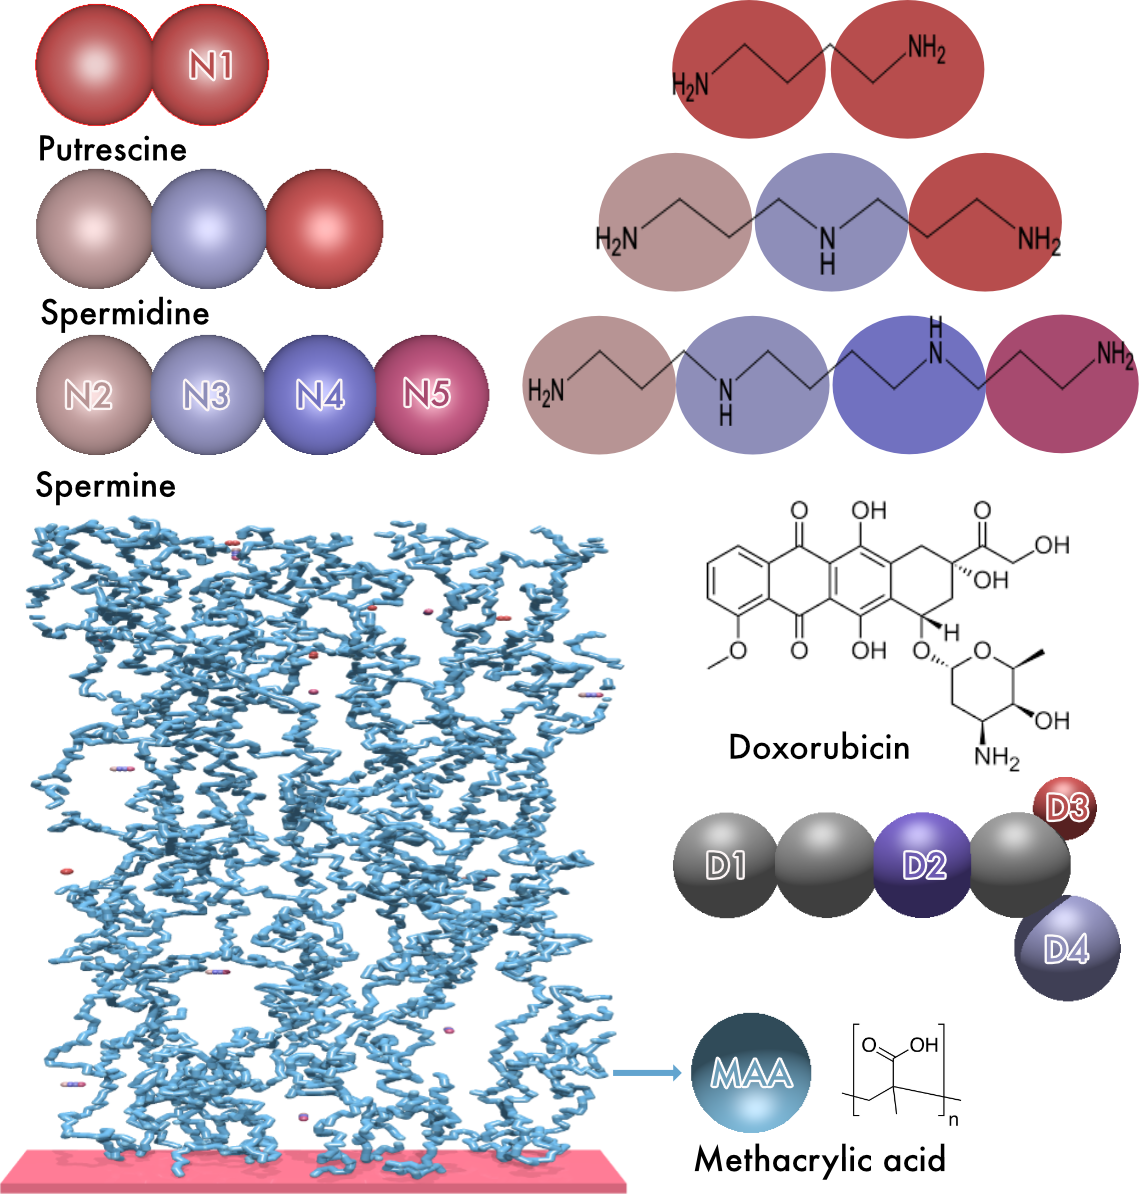
\includegraphics[width=0.7\textwidth]{Figures/graph-film/poliamines_model.png}
	\caption{Esquema del modelo  de  film polim\'erico compuesto por cadenas de MAA. Se muestra adem\'as las poliaminas investigadas  con su respectivo modelo molecular de grano grueso.}
	\label{fig:film:model_poliamines}
\end{figure}





\section{Metodolog\'ia}


El sistema que estudiamos est\'a esquematizado en la figura \ref{fig:film:model_poliamines}.
Consta de una  red de PMAA entrecruzado y anclado en una superficie  la cual est\'a en equilibrio con una soluci\'on que contiene mol\'eculas de agua, iones hidronio e hidr\'oxido, y cloruro de sodio, este \'ultimo est\'a completamente disociado en iones cloruro y sodio.
Adem\'as, esta soluci\'on contiene tanto doxorubicina como una poliamina o ambas especies.
Las poliaminas que hemos considerado son putrescina, espermidina y espermina.

Para estudiar este sistema, aplicamos una teor\'ia molecular que se desarroll\'o recientemente para investigar la absorci\'on en films de hidrogel sensibles al pH de mezclas de prote\'inas \cite{Hagemann2018, longo2019protonation}.
%El enfoque se basa en el trabajo de Szleifer y colaboradores para estudiar el comportamiento de capas de polielectrolitos d\'ebiles injertados  \cite{Nap2006, Gong2007PRL}.
El m\'etodo empleado aqu\'i es general y se puede extender a otros \'ambitos. Por ejemplo, lo hemos aplicado al estudio de la captura de glifosato en hidrogeles de poli(alilamina) \cite{PerezChavez2018} con fines de remediaci\'on ambiental.

A continuaci\'on, presentaremos una descripci\'on de la teor\'ia con \'enfasis en el modelo molecular introducido para describir la doxorubicina, la putrescina, la espermidina y la espermina.


\section{Te\'oria Molecular } \label{sec:film-teoria}

El m\'etodo propuesto consiste en minimizar una energ\'ia libre generalizada que incluye toda la termodin\'amica relevante que engloba los procesos del sistema polim\'erico con una soluci\'on.
Para tal fin  usamos  una descripci\'on molecular de grano grueso de las diferentes especies qu\'imicas que componen el sistema.
Dicha descripci\'on incluye forma, tama\~no, distribuci\'on de carga  y estado de protonaci\'on de cada componente molecular.
Describiremos la fisicoqu\'imica de un film  que  se encuentra en  equilibrio con una soluci\'on acuosa, la cual  tiene una composici\'on  definida externamente (ba\~no de la soluci\'on).
Es decir, el pH, la concentraci\'on de sal y la concentraci\'on de adsorbatos son variables independientes.

\subsection{Formalismo Te\'orico}
Nuestro film que posee distintos tipos de segmentos: un segmento que sirve como entrecruzante entre las cadenas polim\'ericas, el cual es considerado electro-neutral, y  una unidad sensible al pH:  \'acido metacr\'ilico.
Este film  se encuentra en equilibrio con una soluci\'on a temperatura, pH y concentraci\'on de sal definidas. Adem\'as vamos a considerar que en dicha soluci\'on hay un adsorbato, denominado \textit{ads}, el cual puede ser la doxorubicina, o alguna de las poliaminas.
La generalizaci\'on del m\'etodo para incorporar dos o m\'as adsorbatos es relativamente sencilla.
Considerando los aspectos anteriores es posible definir la energ\'ia libre de Helmoholtz:

\begin{align}
 	F = -TS_{mez} -TS_{conf,net} + F_{qca,net} + F_{qca,ads} + U_{elec} + U_{ste} + U_{VDW}
 	\label{eq:film:libre-film}
\end{align}
 
\noindent En donde $S_{mez}$ es la entrop\'ia de traslaci\'on (y de mezcla) de las especies libres: mol\'eculas de agua (H$_2$O), iones:  hidronio (H$_3$O$^+$), e hidr\'oxido (OH$^- $), cationes y aniones de sal y nuestro adsorbato modelo.
Aqu\'i, consideramos una sal monovalente, NaCl, la cual est\'a completamente disociada en sus  iones cloruro (Cl$^-$) y sodio ($Na^+$). 
$S_{conf,net}$ representa la entrop\'ia conformacional que resulta de la flexibilidad de la red polim\'erica, la cual viene dada por todas las conformaciones diferentes que puede asumir.
$F_{qca,net}$, es la energ\'ia qu\'imica libre que describe el equilibrio entre las especies protonadas y desprotonadas de unidades \'acidas. Provenientes de las cadenas de PMAA que forman la red polim\'erica.
De manera similar, $F_{qca,ads}$ describe la protonaci\'on de residuos titulables del adsorbato.
$U_{elec}$ y $U_{ste}$ representan, respectivamente, las interacciones electrost\'aticas y las repulsiones est\'ericas.
Las interacciones de Van der Waals son representadas en $U_{VdW}$.


Las expresiones explicitas de la ecuaci\'on \ref{eq:film:libre-film} las describimos a continuaci\'on.

Como primer t\'ermino tenemos la entrop\'ia de mezcla de  las especies m\'oviles, entre ellas consideramos a nuestro adsorbato: 

\begin{align}
	\begin{aligned}
		-\frac{S_{mez}}{k_B}= &A\sum_{\gamma}\int_0^\infty{dz\rho_\gamma(z)\left(\ln \left(\rho_\gamma (z)v_w\right) -1 + \beta\mu^0_\gamma\right)} \\
		&+ A\sum_{\theta}\int_0^\infty{dz\rho_{ads}(\theta,z)\left(\ln \left(\rho_{ads}(\theta,z)\right) -1 + \beta\mu^0_{ads} \right)}
			\label{eq:film:entropia-mezcla}
	\end{aligned}
\end{align}

\noindent en donde $\beta = \frac{1}{k_B T}$, y $k_B$ es la constante de Boltzmann, $T$ es la temperatura absoluta del sistema. La variable $z$ es la coordenada que mide la distancia a la superficie de soporte de nuestro film, el \'area total de esta superficies es $A$. $\rho_\gamma(z)$ y $\mu^0_\gamma$ es densidad local, a un $z$ dado, y potencial qu\'imico estadar de la especie $\gamma$ respectivamente.
El sub\'indice $\gamma$ toma en cuenta la mol\'ecula de agua e iones hidronio e hidr\'oxido, iones sodio y cloruro.  


El segundo t\'ermino de la ecuaci\'on \ref{eq:film:entropia-mezcla} corresponde a la entrop\'ia de mezcla del adsorbato. $\rho_{ads}(\theta,z)$ es la densidad local del mismo en la conformaci\'on $\theta$. Es decir, $\theta$ recorre sobre las configuraciones del adsorbato.
Esta conformaciones incluyen rotaciones espaciales de la droga/poliamina.
De este modo la densidad local media del adsorbato  puede expresarse como:


\begin{align}
	\left<\rho_{ads}(z)\right> = \sum_\theta{\rho_{ads}(\theta,z)}
	\label{eq:film:ads-z-theta}
\end{align}

\noindent donde $<>$ indica promedio de ensamble sobre configuraciones del adsorbato.
La entrop\'ia conformacional que resulta de la flexibilidad de la red polim\'erica de nuestro film se representa en:

\begin{equation}
	\frac{S_{conf,net}}{k_B} = - \sum_{\alpha}{P(\alpha)\ln P(\alpha)}
\end{equation}

\noindent en donce $P(\alpha)$ denota la probabilidad de que el film se encuentre en la configuraci\'on $\alpha$. Una configuraci\'on viene dada por el conjunto de posiciones de cada uno de los segmentos de la red polim\'erica. 

El siguiente t\'ermino de la ecuaci\'on \ref{eq:film:libre-film} describe  la energ\'ia libre dada por  el equilibrio \'acido-base de los segmentos de MAA que componen la red. 

\begin{align}
	\begin{aligned}
		\beta F_{qca,net} &= A\int_0^\infty dz \left<\rho_{MAA}(z)\right> \left[f(z)(\ln f(z)+ \beta\mu^0_{MAA^-})\right.\\
		&\left.+(1-f(z))(\ln (1-f(z))+\beta\mu^0_{MAAH})\right]    
	\end{aligned}
\end{align} 

\noindent en donde $f(z)$ es el grado de carga de los segmentos de MAA entre  $z$ y $z + dz$. 
$\mu^0_{MAA^-}$ y $\mu^0_{MAAH}$ son los potenciales qu\'imico estandar  de las especies  desprotonadas y protonadas respectivamente.
Adem\'as se define:

\begin{align}
	\left< \rho_{MAA}(z)\right> = \sum_\alpha{P(\alpha)\rho_{MAA}(\alpha,z)}
\end{align}
\noindent donde $\left< \rho_{MAA}(z)\right>$ es la densidad local de segmentos de MAA en promedio de ensamble. $\rho_{MAA}(\alpha,z)$ es la densidad de estos segmentos cuando el pol\'imero se encuentra en una configuraci\'on $\alpha$. Esta \'ultima cantidad es un input de nuestros c\'alculos (para cada configuraci\'on) que debe ser suplido por un modelo molecular complementario al formalismo te\'orico.


%%%%%%%%%%%%%%%%%%%
El equilibrio qu\'imico de las unidades titulables del adsorbato  es considerado en el siguiente t\'ermino de la energ\'ia libre:

\begin{align}
	\begin{aligned}
		\beta F_{qca,ads} = A\int_0^\infty dz& \sum_\tau \left<\rho_{ads,\tau}(z)\right> \left[g_\tau(z)(\ln g_\tau(z)+ \beta\mu^0_{\tau p})\right.\\
		&\qquad\left.+(1-g_\tau(z))(\ln (1-g_\tau(z))+\beta\mu^0_{\tau d})\right]   
	\end{aligned}
\end{align} 

\noindent en donde $\left<\rho_{ads,\tau}(z)\right>$ representa la densidad local promedio del segmento protonable $\tau$ del adsorbato que se define como:

\begin{align}
	\left<\rho_{ads,\tau}(z)\right> = A\sum_\theta \int dz^\prime  \rho_{ads}(\theta,z^\prime)n_\tau(\theta,z^\prime, z)
	\label{eq:film:segments_pro_si}
\end{align}
\noindent en donde $n_\tau(\theta,z^\prime, z)$ es el n\'umero de segmentos $\tau$ entre  $z$ and $z+ dz$ cuando el adsorbato se encuentra en la configuraci\'on $\theta$ y su centro de masa en la posici\'on $z^\prime$.

La unidad titulable puede estar en estado protonado $\tau, p$ o desprotonado $\tau, d$, los cuales poseen su potenciales qu\'imicos est\'andar $\mu^0_{\tau,p}$ y $\mu^0_{\tau,d}$ respectivamente. 
$g_\tau (z)$ es el grado de protonaci\'on de la unidad $\tau$ en $z$. Si $f_\tau (z)$ es el grado de carga local de la unidad, entonces:


\begin{enumerate}
	\item para unidades \'acidas: $g_\tau(z) = 1-f_\tau(z)$ ( las unidades $\tau$ se cargan negativamente)
	\item para unidades b\'asicas: $g_\tau(z) = f_\tau(z)$ (las  unidades $\tau$ se cargan positivamente  )
\end{enumerate}

%%%%%%%%%%

La energ\'ia electr\'ostatica se define como:
\begin{align}
	\begin{aligned}
		\beta U_{elec}= A\int_0^\infty dz&\left[\left(\sum_{\gamma } {\rho_\gamma(z) q_\gamma + \sum_\tau{f_\tau(z) \left<\rho_{ads,\tau}(z)\right> q_\tau} +  f(z)\left<\rho_{MAA}(r)\right>q_{MAA}}\right)\beta\psi(z) \right. \\ &\left.-\frac{1}{2}\beta\epsilon(\nabla\psi(z))^2 \right]
	\end{aligned}
\end{align} 

\noindent en donde $\psi(z)$ es el potencial electrost\'atico dependiente de la posici\'on, $\epsilon$ es la constante de permitividad del medio, $q_\gamma$ es la carga correspondiente a la especie m\'ovil $\gamma$, $q_\tau$ es la carga que adquieren los segmentos titulables del adsorbato. Finalmente $q_{MAA}$ es la carga que adquiere el segmento de $MAA$ al desprotonarse.


En este contexto, la densidad de carga media es:

\begin{align}
	\left<\rho_q(z)\right> = \sum_{\gamma } {\rho_\gamma(z) q_\gamma + \sum_\tau{f_\tau(z) \left<\rho_{ads,\tau}(z)\right> q_\tau} +  f(z)\left<\rho_{MAA}(z)\right>}q_{MAA}
	\label{eq:film:rho_charge}
\end{align}
%%%%%%%%%%%%%%%%

La contribuci\'on siguiente en la energ\'ia libre viene dada por la repulsi\'on est\'erica entre  todos los segmentos que componen  el sistema. Esta contribuci\'on se incorpora a trav\'es de la siguiente restricci\'on:  

\begin{align}
	\begin{aligned}
		1=  {\left[\sum_{\gamma}\rho_\gamma(z) v_\gamma + \sum_\lambda{\left<\rho_{ads,\lambda}(z)\right>v_\lambda} + \left<\rho_{MAA}(z)\right>v_{MAA} \right]},~ \forall z
	\end{aligned}
	\label{eq:film:constraint}
\end{align}
\noindent en donde $v_\gamma$ , $v_\lambda$ y $v_{MAA}$ son los vol\'umenes moleculares de los segmentos $\gamma$ de las especies libres, $\lambda$  en el adsorbato y los segmentos de $MAA$ del pol\'imero respectivamente.
$\left<\rho_{ads,\lambda}(z)\right>$ es definido de la misma forma que en la ecu.  \ref{eq:film:segments_pro_si}.
Cabe destacar que el sub\'indice $\lambda$ considera a todos los segmentos del adsorbato, no solo aquellos titulables, es decir $ \{\tau \}  \in \{\lambda \}$.

%%%%%%%%%%%%%%%
La energ\'ia proveniente de las interacciones de Van der Waals se expresa en el t\'ermino $U_{VdW}$. En este trabajo se ha considerado que todos los segmentos del sistema poseen un car\'acter hidrofilico. Es decir la interacci\'on entre cada par de segmentos es similar a su interacci\'on con las mol\'eculas de agua. Como resultado la energ\'ia de interacci\'on de $VdW$ se considera una constante aditiva a la energ\'ia libre, por lo cual puede ser ignorada. En el cap\'itulo \ref{Chapter-geles} mostraremos un ejemplo en donde las interacciones de $VdW$ son tenidas en cuenta y su efecto es considerable . 

En este punto la energ\'ia libre, ecuaci\'on \ref{eq:film:libre-film}, se puede escribir como una funcional de la probabilidad de distribuci\'on de segmentos de nuestra red polim\'erica, las densidades locales de cada una de las especies libres, incluidas la densidad de conformaciones de la droga y/o polimamina, los grados de protonaci\'on/disociaci\'on y el potencial electrost\'atico local. Es decir:

\begin{align}
	F = \sum_\alpha \sum_\theta \int_0^\infty dz f(\alpha, \theta,z)
\end{align}

\noindent en donde:

\begin{align}
	 f=  f \left( P(\alpha), \{\rho_\gamma(z)\},\rho_{ads}(\theta, z), \{f_\tau(z)\}, f(z), \psi(z)  \right)
	 \label{eq:film:funcionales}
 \end{align}

\noindent de forma m\'as explicita:

\begin{align}
	\begin{aligned}
		\beta F=  & A\sum_{\gamma}\int_0^\infty{dz\rho_\gamma(z)\left(\ln \left(\rho_\gamma (z)v_w\right) -1 + \beta\mu^0_\gamma\right)} \\
		%%%%%
		&+ A\sum_{\theta}\int_0^\infty{dz\rho_{ads}(\theta,z)\left(\ln \left(\rho_{ads}(\theta,z)\right) -1 + \beta\mu^0_{ads} \right)} \\
		%%%%%
		&+ \sum_\alpha{P(\alpha)\ln P(\alpha)} \\
		%%%%
		& + A\int_0^\infty dz \left<\rho_{MAA}(z)\right> \left[f(z)(\ln f(z)+ \beta\mu^0_{MAA^-})\right.\\
		& \qquad\qquad\qquad \left.+(1-f(z))\left(\ln (1-f(z))+\beta\mu^0_{MAAH}\right)\right] \\
		%%%%%
		& + A\int_0^\infty dz \sum_\tau \left<\rho_{ads,\tau}(z)\right> \left[g_\tau(z)(\ln g_\tau(z)+ \beta\mu^0_{\tau p})\right.\\
		&\qquad \qquad \qquad\qquad \qquad\quad \left.+(1-g_\tau(z))(\ln (1-g_\tau(z))+\beta\mu^0_{\tau d})\right]   \\
		%%%%%%%
		 & +A\int_0^\infty dz \left[\left(\sum_{\gamma } {\rho_\gamma(z) q_\gamma + \sum_\tau{f_\tau(z) \left<\rho_{ads,\tau}(z)\right> q_\tau} +  f(z)\left<\rho_{MAA}(r)\right>q_{MAA}}\right)\beta\psi(z) \right. \\ & \qquad \qquad \left.-\frac{1}{2}\beta\epsilon(\nabla\psi(z))^2 \right]
		\end{aligned}
\end{align}


El film est\'a el equilibrio con el bulk de la soluci\'on. Esta soluci\'on posee una composici\'on bien definida (pH, concentraci\'on salina y de adsorbatos) adem\'as de una temperatura absoluta de trabajo. Lo que implica que el sistema est\'a en contacto con un reservorio de part\'iculas libres, lo cual fija los potenciales qu\'imicos de estas especies. Estos potenciales corresponden a las especies libres peque\~nas, $\mu_\gamma$ y del adsorbato, $\mu_{ads}$. Al considerar esta condici\'on de equilibrio qu\'imico el potencial termodin\'amico relevante en el gran potencial: 

\begin{align}
	\begin{aligned}
		\Omega = &F - \sum_\gamma \mu_\gamma N_\gamma -  \mu_{ads} N_{ads} \\
			= &F -\sum_\gamma A\int_0^\infty dz \mu_\gamma \rho_\gamma(z) -  \mu_{ads} N_{ads}  \\
			& \qquad -A\int_0^\infty \mu_{H^+} \left( \sum_\tau\left< \rho_{ads,\tau}(z) \right>g_\tau(z) + (1-f(z))\left< \rho_{MAA}(z) \right> \right )
			\end{aligned}
		\label{eq:film:equil-qco}
\end{align}

\noindent $N_\gamma$ y $ N_{ads}$ son el n\'umero total de mol\'eculas de la especie libre $\gamma$ y adsorbato respectivamente. En la \'ultima linea de la expresi\'on, ecuaci\'on \ref{eq:film:equil-qco}, se tiene en cuenta los protones asociados a las especies con segmentos titulables: adsorbato y red polim\'erica respectivamente.


Se impone una restricci\'on f\'isica adicional a nuestro sistema fluido: las condiciones de equilibrio deben satisfacer la condici\'on de incompresibilidad del sistema: ecu. \ref{eq:film:constraint}.  Esta restricci\'on se incorpora como:

\begin{align}
	\Phi = \Omega +A \int_0^\infty dz\pi(z){\left[\sum_{\gamma}\rho_\gamma(z) v_\gamma + \sum_\lambda{\left<\rho_{ads,\lambda}(z)\right>v_\lambda} + \left<\rho_{MAA}(z)\right>v_{MAA} -1 \right]}
\end{align}


\noindent en donde $\pi(z)$ es un multiplicador local de Lagrange.  Esta funci\'on puede interpretarse como la presi\'on osm\'otica local. Finalmente, se obtiene un nuevo potencial termodin\'amico para nuestro sistema, el cual se escribe de forma explicita como:
 
\begin{align}
	\begin{aligned}
		\beta \Phi=  & A\sum_{\gamma}\int_0^\infty{dz\rho_\gamma(z)\left(\ln \left(\rho_\gamma (z)v_w\right) -1 + \beta\mu^0_\gamma\right)} \\
		%%%%
		&+ A\sum_{\theta}\int_0^\infty{dz\rho_{ads}(\theta,z)\left(\ln \left(\rho_{ads}(\theta,z)\right) -1 + \beta\mu^0_{ads} \right)} \\
		%%%%%%
		&+ \sum_\alpha{P(\alpha)\ln P(\alpha)} \\
		%%%%%%%
		& + A\int_0^\infty dz \left<\rho_{MAA}(z)\right> \left[f(z)(\ln f(z)+ \beta\mu^0_{MAA^-})\right.\\
		& \qquad\qquad\qquad \left.+(1-f(z))(\ln (1-f(z))+\beta\mu^0_{MAAH})\right] \\
		%%%%%%%
		& + A\int_0^\infty dz \sum_\tau \left<\rho_{ads,\tau}(z)\right> \left[g_\tau(z)(\ln g_\tau(z)+ \beta\mu^0_{\tau p})\right.\\
		&\qquad \qquad \qquad\qquad \qquad\quad \left.+(1-g_\tau(z))(\ln (1-g_\tau(z))+\beta\mu^0_{\tau d})\right]   \\
		%%%%%%%
		& +A\int_0^\infty dz \left[\left(\sum_{\gamma } {\rho_\gamma(z) q_\gamma + \sum_\tau{f_\tau(z) \left<\rho_{ads,\tau}(z)\right> q_\tau} +  f(z) \left<\rho_{MAA}(r)\right>q_{MAA}}\right)\beta\psi(z) \right. \\ & \qquad \qquad \left.-\frac{1}{2}\beta\epsilon(\nabla\psi(z))^2 \right] \\ 
		%%%%%%%%
		& +A \int_0^\infty dz\beta\pi(z){\left[\sum_{\gamma}\rho_\gamma(z) v_\gamma + \sum_\lambda{\left<\rho_{ads,\lambda}(z)\right>v_\lambda} + \left<\rho_{MAA}(z)\right>v_{MAA} -1 \right]} \\
		%%%%%%%%%%%
		&   -\sum_\gamma A\int_0^\infty dz \left(\beta \mu_\gamma \rho_\gamma(z) + \beta \mu_{ads} \left<\rho_{ads}(z)\right> \right)  \\
		&  -A\int_0^\infty \beta\mu_{H^+} \left( \sum_\tau\left< \rho_{ads,\tau}(z) \right>g_\tau(z) + (1-f(z)) \left< \rho_{MAA}(z) \right> \right )
	\end{aligned}
\end{align}
 
Obtenido la expresi\'on que define el potencial termodin\'amico del sistema es necesario encontrar las condiciones en las cuales se minimiza el mismo. Para ello se deriva este potencial respecto a los funcionales que lo componen.
A continuaci\'on se mostrara la optimizaci\'on de este gran potencial respecto de los funcionales presentados en  ecu. \ref{eq:film:funcionales}.

En part\'icular la optimizaci\'on respecto a la densidad de las especies libres, $\rho_\gamma (z)$ resulta en:

\begin{align}
	\frac{\partial\beta\Phi}{\partial\rho_\gamma(z)} = 0
\end{align}

Obteni\'endose:
\begin{align}
	\rho_\gamma(z)v_w = a_\gamma \exp\left[-\beta q_\gamma\psi(z)\right] \exp\left[-\beta v_\gamma\pi(z)\right]
	\label{eq:film:free-species}
\end{align}

\noindent en donde la actividad de la especie $\gamma$ se define como:
\begin{align}
	a_\gamma = \exp[\beta\mu_\gamma - \beta\mu^0_\gamma]
\end{align}

En esta expresi\'on se ve la influencia de los potenciales qu\'imicos de las especies libres,  $\mu_\gamma$, los cuales  deben estar en equilibrio con el bulk de la soluci\'on. Las actividades qu\'imicas est\'an completamente determinadas por la composici\'on (pH, concentraci\'on salina) del seno de la soluci\'on.
 
Luego de su correspondiente optimizaci\'on el grado de disociaci\'on de los segmentos de $MAA$ viene dado por:

\begin{align}
	\frac{f(z)}{1-f(z)} = \frac{K^0_{a,MAA}}{a_{H^+}} \exp[-\beta q_{MAA}\psi(z)]
	\label{eq:film:degree-film}
\end{align}

\noindent en donde se la constante termodin\'amica del equilibrio \'acido-base para los segmentos de $MAA$ es:

\begin{align}
	K_{a,MAA}^0 = \exp[-\beta\mu^0_{MAAH} -\beta\mu^0_{MAA^-} -\beta\mu^0_{H^+}]
	\label{eq:film:ka-acido-base}
\end{align}

Del mismo modo para el grado de carga de los segmentos titulables $\tau$, se obtiene:

\begin{align}
	\frac{f_\tau(z)}{1-f_\tau(z)} = \left(\frac{a_{H^+}}{K^0_{a,\tau}}\right)^{\mp 1} \exp[-\beta q_\tau \psi(z)]
	\label{eq:film:degree-protein}
\end{align}


\noindent la constante termodin\'amica para el equilibrio de los segmentos $\tau$ se define:

\begin{align}
	K_{a,\tau}^0 = \exp[-\beta\mu^0_{\tau p} -\beta\mu^0_{\tau d} -\beta\mu^0_{H^+}]
	\label{eq:film:tau-acido-base}
\end{align}

\noindent adem\'as el exponente,$\mp 1$, en la ecuaci\'on \ref{eq:film:degree-protein}, cambia si se trata de segmentos \'acidos ($-$) o b\'asicos ($+$) respectivamente.

Optimizando respecto a la probabilidad de las conformaciones de la red polim\'erica se obtiene:

\begin{align}
	\begin{aligned}
	P(\alpha) = &\frac{1}{Q}\exp\left[ -A \int^\infty_0 \rho_{MAA}(\alpha, z) \ln f(z)\right] \\
	%%%%
	&\exp\left[ -A \int^\infty_0 \rho_{MAA}(\alpha, z) \beta q_{MAA} \psi(z)\right] \\
	& \exp\left[ -A \int^\infty_0 \rho_{MAA}(\alpha, z) \beta v_{MAA} \pi(z)\right] 
	\end{aligned}
	\label{eq:film:probabilidad}
\end{align}

\noindent en donde:
\begin{align}
	\begin{aligned}
		Q = &\sum_\alpha \left\{ \exp\left[ -A \int^\infty_0 \rho_{MAA}(\alpha, z) \ln f(z)\right]\right\} \\
		%%%
		& + \sum_\alpha\left\{ \exp\left[ -A \int^\infty_0 \rho_{MAA}(\alpha, z) \beta q_{MAA} \psi(z)\right]  \right\} \\
		%%%
		& + \sum_\alpha\left\{ \exp\left[ -A \int^\infty_0 \rho_{MAA}(\alpha, z) \beta v_{MAA} \pi(z)\right]  \right\} 
	\end{aligned}
\end{align}

\noindent es la constante con la cual se tiene en cuenta que la sumatoria de las probabilidades de cada conformaci\'on de la red polim\'erica sea 1:

\begin{align}
	\sum_\alpha P(\alpha) = 1                 
\end{align}

Para la densidad local del adsorbato en una conformaci\'on $\theta$ se deriva la siguiente expresi\'on:

\begin{align}
	\begin{aligned}
	\rho_{ads}(\theta, z)v_w = &\tilde{a}_{ads} \prod_\tau\exp\left[-A\int_0^\infty dz^\prime n_\tau(\theta,z,z^\prime) \ln f_\tau(z^\prime)\right] \\
	& \prod_\lambda \exp \left[-A\int^\infty_0 dz^\prime n_\lambda(\theta,z, z^\prime)[v_\lambda\beta\pi(z^\prime) + \beta q_\lambda \psi(z^\prime)] \right]
	\end{aligned}
\label{eq:film:proteina}
\end{align}

En esta expresi\'on se ha redefinido el potencial qu\'imico est\'andar del adsorbato:

\begin{align}
	\tilde{a}^0_{ads} = \exp[\beta\mu_{ads} - \beta\tilde{\mu}^0_{ads}]
	\label{eq:film:actividad-pro}
\end{align}

\noindent en donde se hace la distinci\'on si los segmentos son de naturaleza \'acida $\tau, a$ o b\'asica $\tau,b$:

\begin{align}
	\beta\tilde{\mu}^0_{ads} =  \beta \mu^0_{ads}  + \sum_{\tau,a} C_{n,\tau}\beta\mu^0_{\tau,d} 
	+ \sum_{\tau,b} C_{n,\tau}\beta(\mu_{H^+} - \mu^0_{\tau,p})
\end{align}



\noindent se define el n\'umero de composici\'on, $C_{n,j}$, para un segmento $j$:
\begin{align}
	C_{n,j} = A\int_0^\infty dz \, n_j(\theta, z^\prime, z), \forall z^\prime
	\label{eq:film:n-coord}
\end{align}




La variaci\'on del gran potencial respecto del potencial electrost\'atico que da origen a la ecuaci\'on de Poisson:

\begin{align}
	\epsilon \nabla^2 \Psi(z) = - \left< \rho_q (z)\right>
\end{align}

%%%%
%% qué sentido tiene esto ??
En esta expresi\'on podemos observar  el acoplamiento local entre las interacciones f\'isicas, la organizaci\'on molecular, los grados de libertad, conformaciones y equilibrios qu\'imcos. Para ello hay que tener en cuenta la densidad de carga definida en ecu. \ref{eq:film:rho_charge} 
%%%%

Para la resoluci\'on de nuestro sistema, es decir que el mismo  se encuentre en equilibrio, se han impuesto ciertas restricciones, como la incompresibilidad o equilibrio de potenciales qu\'imicos ecuaciones \ref{eq:film:constraint} y \ref{eq:film:equil-qco} respectivamente. Otra restricci\'on que se impone es la electro neutralidad global del sistema. Es decir:

\begin{align}
	\int_0^\infty dz \left< \rho_q (z)\right> = 0
\end{align}

Esta restricci\'on se satisface en la soluci\'on a la ecuaci\'on de Poisson al considerar las condiciones de contorno adecuadas, las cuales definimos:

\begin{align}
	\begin{aligned}
		&i)  \lim_{z\to\infty}\psi(z) = 0 \\
		&ii) \left.\frac{d\psi(z)}{dz}\right|_{z=0} = 0
		\label{eq:film:contorno}
	\end{aligned}
\end{align}

Estas condiciones significan que el potencial electrost\'atico se desvanece a medida que nos alejamos de nuestro film polim\'erico.

En este punto hemos mostrados las expresiones que optimizan a nuestro gran potencial, y c\'omo cada uno de estas funciones: $P(\alpha), \rho_\gamma(z),\rho_{ads}(z), f_\tau(z), f(z), \psi(z) $ a su vez  terminan siendo definidos por dos potenciales locales: Electrost\'atico $\psi(z)$ y Presi\'on osm\'otica $\pi(z)$, las actividades de las especies libres y algunas otras cantidades, que son variables conocidas del sistema.
Con las condiciones del ba\~no de la soluci\'on: concentraci\'on de sal, el pH, y concentraci\'on de adsorbato es posible calcular las actividades de todas las especies libres considerando las incompresibilidad del sistema y su eletro-neutralidad, as\'i como tambi\'en la auto-disociaci\'on del agua.  
Las variables conocidas del sistema incluyen el volumen molecular y carga de cada una de las especies libres presentes, las constantes de disociaci\'on de los segmentos titulables, as\'i como tambi\'en la distribuci\'on espacial de todos los segmentos para cada una de las conformaciones que tome el film y/o adsorbatos. Todas estas cantidades son provistas por un modelo molecular. Este modelo molecular ser\'a descrito m\'as adelante en la secc\'on \ref{sub:film:modelo-molecular}.

Con esas consideraciones vemos que nuestras funciones desconocidas son  $\psi(z)$ y $\pi(z)$ las cuales pueden ser determinadas por sustituci\'on en la diferentes ecuaciones en las que interact\'uan: la densidad de las especies libres ecuaci\'on  \ref{eq:film:free-species}, los grados de disociaci\'on de los segmentos del film y de los  titulables del adsorbato ecuaciones \ref{eq:film:degree-film} y \ref{eq:film:degree-protein} respectivamente, la probabilidad de las conformaciones de la red polim\'erica ecu. \ref{eq:film:probabilidad} y la densidad local del adsorbato  ecuaci\'on \ref{eq:film:proteina}.

Una vez obtenidos los potenciales $\pi(z)$ y $\psi(z)$ es posible derivar  cualquier cantidad termodin\'amica de inter\'es  a partir de la energ\'ia libre o haciendo uso de alguna expresi\'on explicita en base a las funciones definidas anteriormente.

Por ejemplificar la fracci\'on de volumen local ocupada por un adsorbato puede ser calculada como:

\begin{align}
	\left< \phi_{ads}(z) \right> = A\int_0^\infty dz^\prime \sum_\theta \rho_{ads}(\theta, z^\prime)\sum_\lambda n_\lambda(\theta, z^\prime, z)v_\lambda
\end{align}

Con esta cantidad es posible cuantificar la adsorci\'on del adsrobato en el film. 

\subsection{Soluci\'on Bulk}\label{sec:film:bulk-solution}

Como mencionamos en la secci\'on anterior, el sistema de estudio est\'a en equilibrio con un reservorio de pH, temperatura y concentraci\'on de las especies libres (incluido el adsorbato). La composici\'on de la soluci\'on bulk nos proporciona la informaci\'on de las actividades de las especies m\'oviles, y con ellas sus potenciales qu\'imicos.

El potencial termodin\'amico que describe a la soluci\'on bulk puede expresarse de la siguiente manera: 


\begin{align}
	\begin{aligned}
		\beta\frac{ \Phi^b}{V}=  & \sum_{\gamma}{\rho^b_\gamma\left(\ln \left(\rho^b_\gamma v_w\right) -1 + \beta\mu^0_\gamma\right)} \\
		%%%%
		&+ \sum_{\theta}{\rho^b_{ads}(\theta)\left(\ln \left(\rho^b_{ads}(\theta)\right) -1 + \beta\mu^0_{ads} \right)} \\
		%%%%%%
		& + \sum_\tau \left<\rho^b_{ads,\tau}\right> \left[g^b_\tau(\ln g^b_\tau+ \beta\mu^0_{\tau p}) +(1-g^b_\tau)(\ln (1-g^b_\tau)+\beta\mu^0_{\tau d})\right]   \\
		%%%%%%%
		& +\left[\left(\sum_{\gamma } {\rho^b_\gamma q_\gamma + \sum_\tau{f^b_\tau \left<\rho^b_{ads,\tau}\right> q_\tau} }\right)\beta\psi^b  \right] \\ 
		%%%%%%%%
		& +\beta\pi^b{\left[\sum_{\gamma}\rho^b_\gamma v_\gamma + \sum_\lambda{\left<\rho^b_{ads,\lambda}\right>v_\lambda}  -1 \right]} \\
		%%%%%%%%%%%
		&   -\sum_\gamma \left(\beta \mu_\gamma \rho^b_\gamma + \beta \mu_{ads} \left<\rho^b_{ads}\right> \right)   -\beta\mu_{H^+} \left( \sum_\tau\left< \rho^b_{ads,\tau} \right>g_\tau  \right )
	\end{aligned}
	\label{eq:film:pot-bulk}
\end{align}

\noindent en donde el super\'indice $b$ denota el Bulk de la soluci\'on. 
Las densidades de cada una de las especies libres es obtenida del limite  $z \to \infty$:

\begin{align}
	\begin{aligned}
		& i)\rho^b_\gamma =\rho_\gamma (z \rightarrow \infty)   \\
		& i)\rho^b_{ads} =\rho_{ads} (z \rightarrow \infty)   \\
		& ii)  \pi^b = \pi(z \rightarrow \infty) \\
		& iii) g_\tau^b = g_\tau(z \rightarrow \infty)  
	\end{aligned}
\end{align}
\noindent en donde $i$ hace referencia a las especies libres y al adsorbato. 

Adem\'as el promedio de ensamble de la densidad del adsorbato definido en la ecuaci\'on \ref{eq:film:ads-z-theta} se convierte en:
\begin{align}
	\left<\rho^b_{ads}\right> = \sum_{\theta}\rho^b_{ads}(\theta)
\end{align}

en consecuencia para las especies libres $\gamma$ resulta:
\begin{align}
	\rho^b_\gamma v_w = a_\gamma \exp\left[ -\beta q_\gamma \psi^b -\beta \pi^b v_\gamma \right]
	\label{eq:film:rhofree-bulk}
\end{align}

El grado de disosiaci\'on de los segmentos $\tau$ titulables del adsorbato:
\begin{align}
		\frac{f^b_\tau}{1-f^b_\tau} = \left(\frac{a_{H^+}}{K^0_{a,\tau}}\right)^{\mp 1} \exp[-\beta q_\tau \psi^b]
\end{align}


finalmente para la densidad del adsorbato se obtiene:

\begin{align}
	\begin{aligned}
		\rho_{ads}(\theta)v_w = &\tilde{a}_{ads} \prod_\tau \exp\left[-Cn_\tau \ln f^b_\tau\right] \\
		& \prod_\lambda \exp \left[-cn_\lambda (v_\lambda\beta\pi^b + q_\lambda \psi^b) \right]
	\end{aligned}
	\label{eq:film:rhopro-bulk}
\end{align}

\noindent en donde $\tilde{a}_{ads}$ y $C_{n,\tau}$ (y $C_{n,\lambda}$) son definidos en las ecuaciones  \ref{eq:film:actividad-pro} y \ref{eq:film:n-coord} respectivamente. 

Podemos observar nuevamente que estas cantidades  quedan en funci\'on de la presi\'on osm\'otica $\pi^b$ y el potencial electrost\'atico $\psi^b$ del bulk.

Sin embargo si consideramos las condiciones de contorno dada en la ecu. \ref{eq:film:contorno} para la ecuaci\'on de Poisson, vemos que en la soluci\'on bulk se debe cumplir: $\psi^b = 0$. 

Finalmente para nuestro ba\~no de soluci\'on las  inc\'ognitas a resolver son la presi\'on osm\'otica, $\pi^b$, y la electro-neutralidad del medio. 
\begin{align}
	\sum_\gamma{\rho^b_\gamma q_\gamma} + \sum_\tau{f_\tau(z) \left(\rho^b_{ads,\tau}\right) q_\tau} = 0
	\label{eq:film:neutralidad-bulk}
\end{align}

Las cuales es posible obtenerlas por resoluci\'on num\'erica al sustituir las ecuaciones  \ref{eq:film:rhofree-bulk} y
 \ref{eq:film:rhopro-bulk}  y sus respectivas actividades (ecuaciones \ref{eq:film:act-bulk-free} y \ref{eq:film:act-bulk-pro} ) en la ecuaci\'on \ref{eq:film:neutralidad-bulk} y la condici\'on de incompresibilidad del bulk de la soluci\'on dada por:

\begin{align}
	\sum_\gamma \rho^b_\gamma v_\gamma + \sum_\lambda\left< \rho^b_{ads,\lambda}\right> v_\lambda = 1
	\label{eq:incom-bulk}
\end{align}

Como se mencion\'o al inicio de esta secci\'on la resoluci\'on del bulk de la soluci\'on, en concreto el c\'alculo de $\pi^b$, nos provee la informaci\'on para las actividades de las especies m\'oviles:

\begin{align}
	a_\gamma =\frac{\rho^b_\gamma v_w}{\exp\left[-\beta \pi^b v_\gamma \right]}
	\label{eq:film:act-bulk-free}
\end{align}

 y para el adsorbato:

\begin{align}
	\begin{aligned}
		\tilde{a}_{ads} = & \rho_{ads}(\theta)v_w\exp\left[cn_\tau \ln f^b_\tau\right] \\
		& \exp \left[cn_\lambda (v_\lambda\beta\pi^b) \right]
	\end{aligned}
\label{eq:film:act-bulk-pro}
\end{align}


Hay que tener en cuenta que las densidades en el bulk de la soluci\'on son par\'ametros de entrada en cada c\'alculo. Una vez que se establecen el pH, la concentraci\'on de sal y de nuestra droga y/o poliamina, estas densidades pueden ser determinadas (usando la electro-neutralidad de la soluci\'on del bulk y la auto-disociaci\'on de equilibrio del agua).


%%%%%%%%%%%%%%%%%%%%%%%%%%%%%%%%%%%%%%%%%

%%%%%%%%%%%%%%%%%%%%%%%%%%%%%%%%%%%%%%

\subsection{Modelo molecular}
\label{sub:film:modelo-molecular}


\begin{figure}[ht]
	\centering
	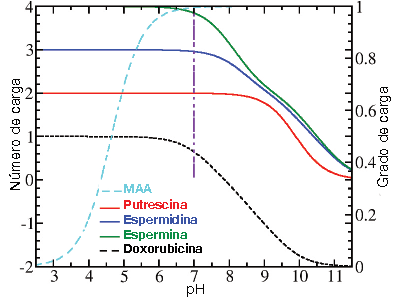
\includegraphics[width=0.45\textwidth]{Figures/graph-film/chargeAds.pdf}
	\caption{N\'umero promedio de carga neta de la doxorrubicina y las poliaminas en funci\'on del pH en soluciones diluidas.
		El eje derecho muestra el grado de carga de una unidad de \'acido metacr\'ilico aislado. La l\'inea vertical punteada indica el pH fisiol\'ogico.}
	\label{fig:film:model}
\end{figure}


Este formalismo te\'orico requiere una representaci\'on molecular de todas las especies qu\'imicas en el sistema. La figura \ref{fig:film:model_poliamines} incluye el esquema de grano grueso utilizado para el MAA y las especies en soluci\'on. Las poliaminas (putrescina, espermidina y espermina) se representan utilizando sus diferentes grupos amino (N1 a N5). El modelo de doxorubicina incluye los anillos (D1, D2 y D4) as\'i como el grupo carbox'ilico (D3). El volumen, pKa y carga de estos grupos, al igual que los de las mol\'eculas de agua e iones, se presentan en la tabla \ref{table:CG}. Las geometr\'ias moleculares, as\'i como los valores de pKa asignados a las diferentes unidades de grano grueso, se han obtenido de la literatura \cite{agostinelli2010polyamines,casero2009recent,puchem}.

La red polim\'erica est\'a compuesta por cadenas entrecruzadas de 50 segmentos de longitud; cada segmento de cadena es una representaci\'on de grano grueso de una unidad de MAA (ver la figura \ref{fig:film:model_poliamines}). Esta red tiene una topolog\'ia similar a la de un diamante, con las unidades de entrecruzamiento con una coordinaci\'on igual a cuatro  \cite{Mann2005,QuesadaPerez2012M,Kosovan2015,Hofzumahaus2018}. Las conformaciones de la red se generan mediante simulaciones de din\'amica molecular. El set de configuraciones fueron obtenidas de un trabajo anterior, realizado en el mismo grupo de investigaci\'on. Como puede verse en la referencia  \cite{Hagemann2018}.



Con el esquema de pKa descrito anteriormente, la figura \ref{fig:film:model} muestra la carga el\'ectrica promedio de cada poliamina y la de la doxorubicina. El gr\'afico tambi\'en muestra el grado de carga de un mon\'omero de MAA aislado en una soluci\'on diluida. La fuerza impulsora para la adsorci\'on, de nuestros adsorbatos en el film,  son las atracciones electrost\'aticas entre la poliamina/droga y el MAA. La carga positiva de todos los adsorbatos disminuye con el aumento del pH. El pol\'imero se vuelve m\'as negativamente cargado a medida que aumenta el pH. Por lo tanto, esperamos que la adsorci\'on sea una funci\'on no monot\'onica del pH de la soluci\'on. Adem\'as, el punto isoel\'ectrico de la doxorubicina se encuentra alrededor del pH neutro, lo que implica que el f\'armaco es neutro en cuanto a carga en condiciones fisiol\'ogicas y tiene carga negativa a valores de pH m\'as altos.



\begin{table}[!ht]
	\begin{centering}
		\centering
		%\footnotesize
		\setlength{\tabcolsep}{2.2pt}
		\begin{tabular}{|cccc|}
			\hline 
			\hspace{0pt}CG unit   & $pKa$ & $q$  & $v$ ($\text{nm}^3$)  \\ \hline
			$N_1$& 9.9 & (+1) &0.051\\
			$N_2$& 10.9& (+1) & 0.051\\ 
		     $N_3$& 8.4& (+1)& 0.063\\
		     $N_4$&7.9& (+1) & 0.063\\
		     $N_5$& 10.1& (+1)& 0.051\\
		      $D_1$&  - & 0 &0.085\\
		     $D_2$& 7.34 & (-1) & 0.085\\ 
			 $D_3$&  8.46& (-1)& 0.035\\
			$D_4$&  9.46 & (+1) &0.085\\ 
			$MAA$&  4.65 & (-1) & 0.065\\
			$H_2O$ & - & 0 & 0.03\\
			$H_3O^+$ & - & +1 & 0.03\\
			$OH^-$ & - & -1 & 0.03\\
			$Na^+$ & - & +1 & 0.033\\ 
			$Cl^-$ & - & -1 & 0.033\\ \hline
		\end{tabular}		
		\caption{Modelo de grano grueso. Los valores de pKa asignados a las diferentes unidades de grano grueso se obtuvieron todos de la literatura \cite{agostinelli2010polyamines,casero2009recent,puchem}, y los vol\'umenes moleculares corresponden a los valores de Van der Waals. Valores entre paracentesis \footnotesize{()} indican la carga de las especies qu\'imicas ionizadas.}
		\label{table:CG}
	\end{centering}
\end{table}

%%%%%%%%%%%%%%%%%%%%%%%%%%%%%%%%%%%%%%%%%%


\begin{figure*}[!htb]
	\centering
	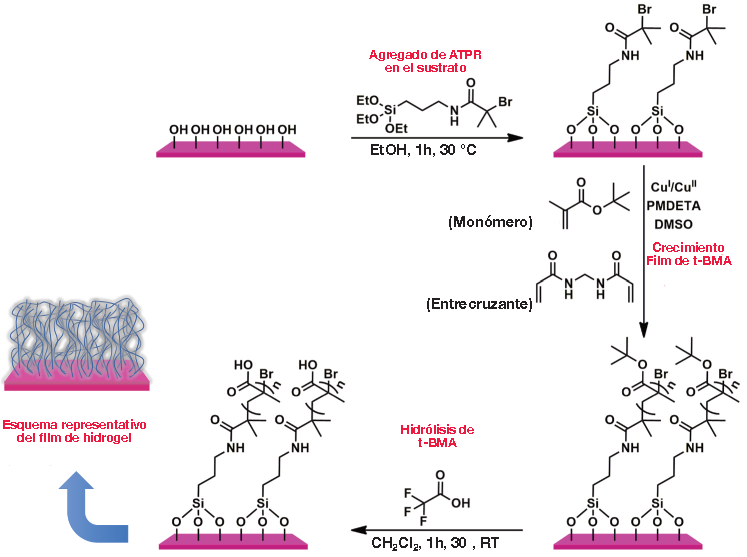
\includegraphics[width=0.7\textwidth]{Figures/graph-film/exp_synt_scheme.pdf}
	\caption{Pasos de la s\'intesis de la pel\'icula delgada de PMAA, representados como: A) Iniciador ATRP en sustratos; B) Crecimiento de la pel\'icula de t-BMA; C) Hidr\'olisis del t-BMA.}
	\label{fig:film:synthesis_scheme}
\end{figure*}




\section{Validaci\'on experimental}


Con el fin de respaldar la teor\'ia y el modelado molecular, se prepararon films de hidrogel polim\'ericos de PMAA y se llevaron a cabo experimentos de carga y liberaci\'on de doxorubicina en presencia de espermina y espermidina. %El \'angulo de contacto del film se midi\'o en cada paso para seguir el procedimiento de s\'intesis, presentados en las siguientes secciones.
Los resultados aqu\'i presentados se realizaron en colaboraci\'on con el grupo de investigaci\'on.



\subsection{Crecimiento controlado de pel\'iculas delgadas de PMAA.}

Los films  de PMAA se obtuvieron mediante la t\'ecnica de Polimerizaci\'on Radical por Transferencia de \'Atomo (ATRP por sus siglas en ingl\'es ), que permite la polimerizaci\'on iniciada en la superficie.
La s\'intesis completa de la pel\'icula de PMAA consta de tres pasos principales, como se representa en la figura \ref{fig:film:synthesis_scheme}. Estos pasos son los siguientes:
1) Inmovilizaci\'on del iniciador de ATRP en los sustratos (portaobjetos de vidrio y obleas de silicio de un solo pulido).
2)Procedimiento de ATRP utilizando ter-butil metacrilato (t-BMA) y N,N'-Metilenbisacrilamida (BIS) como agente de entrecruzante
3)Hidr\'olisis de los films resultantes de ter-butil metacrilato entrecruzado con \'acido trifluoroac\'etico para obtener las pel\'iculas de PMAA.


\emph{1) Inmovilizaci\'on del iniciador de ATRP en los sustratos.}
 Despu\'es de limpiar con agua jabonosa, etanol y acetona en un ba\~no ultras\'onico, los portaobjetos de vidrio y las obleas de silicio se modificaron mediante inmersi\'on en una soluci\'on al 2\% v/v de 2-bromo-2-metil-N-(3-(tri-etoxisilil)propil)propenamida (preparada seg\'un lo informado previamente \cite{Yameen2008}) en etanol seco durante 1 hora a $30^\circ C$. Luego, los sustratos se lavaron con etanol y se curaron durante 2 horas en un horno $60^\circ C$ bajo vac\'io. El \'angulo de contacto medido (goni\'ometro de\'angulo de contacto Ramè-Hart modelo 290) utilizando agua fue de alrededor de $63.6^\circ \pm 0.1^\circ$ sin cambios con el tiempo, ligeramente menor que el del portaobjetos de vidrio ($64.7^\circ \pm 0.2^\circ$).% El conjunto completo de mediciones se muestra en el \SuppInfo (\SI).




\emph{2) Crecimiento de la pel\'icula de ter-butil metacrilato.}
 Las polimerizaciones de ATRP se llevaron a cabo de acuerdo con \cite{Brown2009}. Se prepar\'o una soluci\'on de t-BMA (15 ml, 92 mmol, Aldrich 98\%), BIS (422 mg, 2.76 mmol, Aldrich 99\%), CuBr$_2$ (4.1 mg, 0.018 mmol, Aldrich 99.999\%), y N,N,N,N,N-Pentametildietilentriamina (PMDETA, 0.12 ml, 0.55 mmol, Aldrich, 99\%) disuelta en DMSO (15 ml) y se desgasific\'o mediante burbujeo de N$_2$ durante una hora a temperatura ambiente. Luego, se agreg\'ow CuBr (26.5 mg, 0.18 mmol, Aldrich 99.999\%) y la mezcla se dej\'o bajo N$_2$ durante 15 minutos. Simult\'aneamente, los sustratos con iniciador se sellaron en tubos Schlenk y se desgasificaron mediante ciclos de vac\'io/N$_2$. Luego, la mezcla de reacci\'on se inyect\'o en estos tubos Schlenk para cubrir completamente las muestras. La mezcla se dej\'o reposar durante 24 horas bajo N$_2$, y luego se retiraron los sustratos y se lavaron con DMSO, acetona y se secaron con N$_2$. El \'angulo de contacto medido fue de $89.3^\circ \pm 0.1^\circ$ sin cambios con el tiempo.

\emph{3) Hidr\'olisis del ter-butil metacrilato entrecruzado obtenido.}
 Las pel\'iculas entrecruzadas de PtBMA se sumergieron en una soluci\'on de \'acido trifluoroac\'etico (Aldrich 99\%) en CH$_2$Cl$_2$ (50\% v/v) durante una hora a temperatura ambiente. Luego, los sustratos se lavaron varias veces con agua y se dejaron sumergidos en agua durante 10 minutos antes de secarlos con N$_2$. El \'angulo de contacto medido utilizando agua disminuy\'o con el tiempo, desde un valor inicial de alrededor de 69$^\circ$ hasta 63$^\circ$; este comportamiento indica una exitosa hidr\'olisis de la pel\'icula de PtBMA en una pel\'icula de PMAA m\'as hidrofílica, exponiendo grupos carbox\'ilicos, que se hinchan/hidratan con el tiempo.


\begin{figure*}[htb]
	\centering
	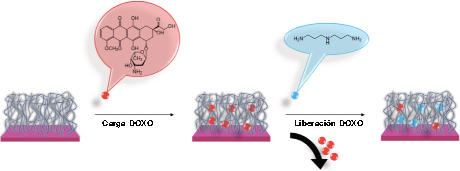
\includegraphics[width=0.7\textwidth]{Figures/graph-film/exp_doxo_load_scheme.pdf}
	\caption{Esquema que muestra la carga de doxorrubicina en el film de hidrogel de PMAA y su liberaci\'on en presencia de espermidina.}
	\label{fig:film:exp_doxo_scheme}
\end{figure*}



\subsection{Captura y liberaci\'on de doxorrubicina en presencia de poliaminas}


La carga de doxorrubicina (Doxo, Aldrich 98.0-102.0\% en clorhidrato de doxorrubicina) se realiz\'o sumergiendo las pel\'iculas de PMAA en una soluci\'on de la droga al $10^{-2}$ M en agua ultrapura \textit{Milli-Q} ($18.2 M \Omega \, cm$) durante 24 horas en el refrigerador (ver figura \ref{fig:film:exp_doxo_scheme}). Se utilizaron las bandas de absorci\'on de Doxo en el rango de 450-550 nm para caracterizar su carga en el film utilizando un espectrofot\'ometro Lambda 35 de Perkin Elmer. Para ello, despu\'es de la carga, los sustratos se sumergieron durante unos segundos en agua ultrapura para eliminar las mol\'eculas adheridas a la superficie y se secaron con un flujo de N2. Finalmente, los sustratos se colocaron verticalmente en el camino \'optico del espectrofot\'ometro y se realizaron los an\'alisis, abarcando el rango de 200-800 nm, con una velocidad de escaneo de 480 nm/min y un ancho de ranura de 1 nm.

La liberaci\'on se realiz\'o sumergiendo los sustratos cargados en agua o en soluciones de espermidina (Aldrich$ >$ 99\%) o espermina (Aldrich $>$ 97\%), cada una al 2.8\% en peso/volumen (ver figura \ref{fig:film:exp_doxo_scheme}) en diferentes momentos. La liberaci\'on se sigui\'o de la misma manera que la carga. Estas soluciones de poliaminas se neutralizaron con hidr\'oxido de sodio al 0.1 M, lo que aument\'o la fuerza i\'onica desde el agua pura y llev\'o a un pH final de 7. Todos los experimentos se realizaron utilizando agua ultrapura \textit{Milli-Q}. La concentraci\'on de poliamina se eligi\'o para explorar un r\'egimen de saturaci\'on, equivalente al extremo de la regi\'on explorada en las predicciones te\'oricas (ver m\'as abajo). De esta manera, se pueden comparar cualitativamente las cantidades de carga de amina equivalentes.

%%%%%%%%%%%%%%%%%%





%%%%
\section{Resultados} \label{sec:film:resultados}

\subsection{Resultados te\'oricos}

La primera pregunta que abordamos es c\'omo responden los hidrogeles de PMAA a las soluciones de poliaminas. El enfoque termodin\'amico permite considerar la absorci\'on dentro de la red polim\'erica a partir de soluciones que contienen estas aminas. Definimos la adsorci\'on como:

\begin{align}
	\begin{aligned}
		\Gamma_i= \int_0^\infty{(\rho_i(z) -\rho_i^{bulk})dz}
	\end{aligned}
	\label{eq:film:adsorption}
\end{align}


\noindent Donde la coordenada $z$ mide la distancia desde la superficie que sostiene al film, y el sub\'indice $i$ se refiere al absorbato de inter\'es. 
La funci\'on local $\rho_{ads}(z)$ es la densidad del absorbato, y $\rho_{ads}^b=\lim_{z\to\infty} \rho_{ads}(z)$ es la densidad en la soluci\'on bulk, lejos del film  de hidrogel. 

Esta definici\'on de $\Gamma$ cuantifica la masa de mol\'eculas absorbidas por unidad de \'area en exceso de la contribuci\'on impuesta por la soluci\'on bulk en equilibrio con el film.

La expresi\'on dada por la ecu. \ref{eq:film:adsorption} describe la absorci\'on de cada una de las aminas, pero tambi\'en es v\'alida para la doxorrubicina.


\begin{figure}[!htb]
	\centering
	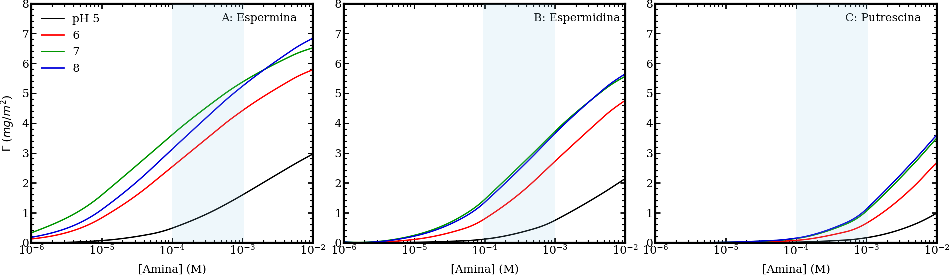
\includegraphics[width=0.9\textwidth]{Figures/graph-film/amines_ads.pdf}
	\caption{Gr\'afico de la adsorci\'on, $\Gamma$, de espermina (A), espermidina (B) y putrescina (C) en funci\'on de su concentraci\'on en la soluci\'on bulk.
		Las diversas curvas en cada panel corresponden a diferentes valores de pH (alrededor de $7$) y condiciones de sal fisiol\'ogica, $[NaCl]=100 ,mM$. Las regiones sombreadas indican el rango de concentraciones saludables de poliaminas \cite{Soda2011}.
		No hay doxorrubicina en estas soluciones.}
	\label{fig:film:amines-ads}
\end{figure}




La figura  \ref{fig:film:amines-ads} muestra las isotermas de absorci\'on para cada una de las poliaminas en funci\'on de su concentraci\'on en la soluci\'on en el bulk. Debido a que existen informes que indican que los alrededores de las c\'elulas tumorales son \'acidos \cite{vaupel1989blood,Tannock1989,Raghunand1999, rofstad2006acidic, schmaljohann2006thermo, Koltai2016}, se incluyen isotermas de absorci\'on para diferentes valores de pH. Enfatizamos que el primer objetivo es investigar la capacidad de los hidrogeles de PMAA para secuestrar poliaminas en condiciones fisiol\'ogicas; luego, los resultados de la figura \ref{fig:film:amines-ads} corresponden a soluciones en ausencia de doxorrubicina y con $100 \, mM$ de $[NaCl]$. La adsorci\'on aumenta con la concentraci\'on creciente de poliaminas. %Esto indica que se alcanza un r\'egimen no saturado con la concentraci\'on explorada, como se puede ver f\'acilmente en las isotermas de absorci\'on.

en la cercania de las c\'elulas sanas, la concentraci\'on de poliaminas se encuentra en el rango de $10^{-4}$ a $10^{-3}\, M$, lo que puede aumentar en un orden de magnitud o m\'as alrededor de los tumores \cite{Soda2011}. Los resultados de la figura \ref{fig:film:amines-ads} sugieren que los hidrogeles de PMAA pueden responder a estas condiciones capturando cantidades crecientes de aminas. En particular, la putrescina muestra un comportamiento aparentemente de encendido/apagado en torno a la transici\'on entre las concentraciones saludables a patol\'ogicas. Adem\'as, excepto para las soluciones m\'as \'acidas (pH 5), este comportamiento de absorci\'on se mantiene para diferentes valores de pH en torno a las condiciones fisiol\'ogicas, lo que se\~nala  la capacidad del hidrogel para adaptarse a peque\~nos cambios de pH causados por c\'elulas da\~nadas.

Las poliaminas adsorbidas se distribuyen de manera m\'as o menos homog\'enea dentro de la pel\'icula de hidrogel. Sin embargo, esta distribuci\'on est\'a correlacionada con la densidad del pol\'imero: se encuentran concentraciones m\'as altas de poliamina en las regiones de fracci\'on de volumen localmente alta de PMAA. Por lo tanto, las poliaminas tienen una mayor probabilidad de encontrarse cerca de las intersecciones de la red, donde ocurre la mayor densidad de pol\'imero. Un comportamiento similar ha sido predicho por  \citet{Sai2020} mediante simulaciones de din\'amica molecular, quienes sugirieron que los anf\'ifilos de crom\'oforos se autoensamblan en los nodos de hidrogeles polielectrol\'iticos entrecruzados qu\'imicamente.


En condiciones similares, el hidrogel absorbe m\'as espermina que espermidina y putrescina (compare los paneles A, B y C de la fig.  \ref{fig:film:amines-ads}, respectivamente), lo que se puede explicar sobre la base de la carga positiva neta de las poliaminas: cuanto m\'as cargada se encuentre la amina, m\'as se absorber\'a en el film porque una carga positiva m\'as alta reduce el costo entr\'opico de la confinaci\'on del contrai\'on al tiempo que permite las atracciones electrost\'aticas con el pol\'imero de MAA.

\citet{Schimka2017} han estudiado la interacci\'on entre microgeles de pol\'imero y surfactantes fotosensibles con poliaminas sint\'eticas como grupos principales. Estos surfactantes tienen diferentes n\'umeros de grupos amino con cargas entre $+1$ y $+3$. Los microgeles ani\'onicos se deshinchan cuando se exponen a una concentraci\'on suficientemente alta de surfactante (dependiendo del estado de isomerizaci\'on del surfactante). Su estudio muestra tanto experimental como te\'oricamente que se necesita una mayor concentraci\'on de surfactante para desencadenar el deshinchamiento de los microgeles cuando se reduce la carga del grupo principal de poliamina. Este comportamiento indica que aumentar el n\'umero de grupos amino facilita la captaci\'on del surfactante por parte del microgel, en acuerdo con los resultados aqu\'i presentados.




\begin{figure}[!htb]
	\centering
	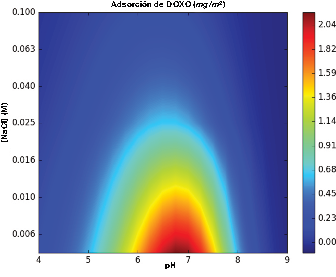
\includegraphics[width=0.5\textwidth]{Figures/graph-film/doxo_load.pdf}
	\caption{Mapa de color que muestra la absorci\'on de la doxorrubicina (ver ecuaci\'on \ref{eq:film:adsorption}) en funci\'on de la composici\'on de la soluci\'on, es decir, el pH y $[NaCl]$; la concentraci\'on del f\'armaco en la soluci\'on es $[Doxo]=1 \, mM$.}
	\label{fig:film:doxo-load}
\end{figure}


A continuaci\'on, consideramos la capacidad de las pel\'iculas de hidrogel de PMAA para incorporar doxorrubicina (Doxo). Los hidrogeles de cadenas de poli\'acido entrecruzadas son sensibles a cambios en la fuerza i\'onica de la soluci\'on o la concentraci\'on de sal \cite{zhang2000}. Este comportamiento puede no ser relevante en entornos biol\'ogicos con una concentraci\'on de iones altamente regulada. Sin embargo, controlar la concentraci\'on de sal es fundamental en el laboratorio para aumentar la carga del agente terap\'eutico dentro del material. Por lo tanto, hemos considerado la absorci\'on de doxorrubicina en condiciones de laboratorio t\'ipicas, abarcando un amplio rango de pH y $[NaCl]$. 

La figura  \ref{fig:film:doxo-load} muestra la absorci\'on en exceso de Doxo, calculada utilizando la ecu. \ref{eq:film:adsorption}. Esta figura resalta el efecto de la disminuci\'on de la salinidad para aumentar la absorci\'on del f\'armaco. Debido a que la carga de la doxorrubicina es $+1$ (a bajo pH), su absorci\'on compite con la de los iones de sodio para neutralizar la carga del pol\'imero. Por lo tanto, las mejores condiciones para su incorporaci\'on en la pel\'icula corresponden a la reducci\'on de la disponibilidad de iones  de sal.


\begin{figure}[!htb]
	\centering
	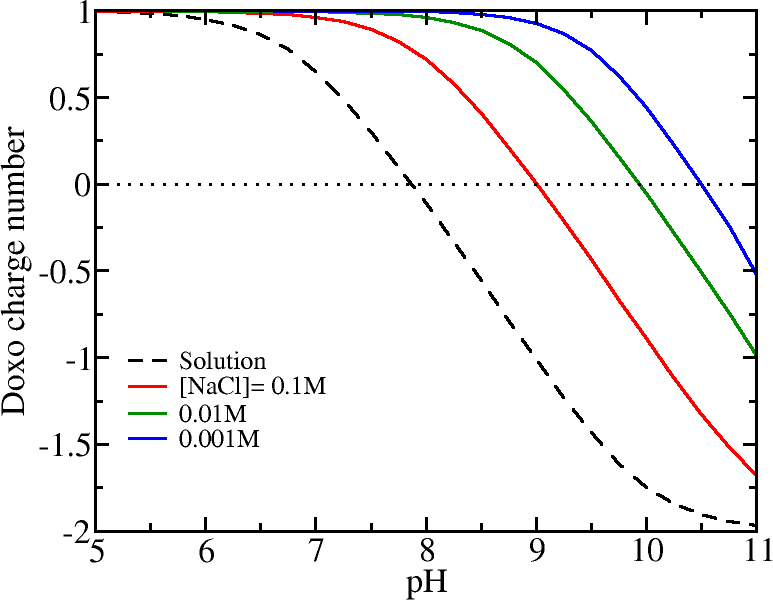
\includegraphics[width=0.45\textwidth]{Figures/graph-film/doxo-charge.png}
	\caption{Gr\'afico que muestra el n\'umero de carga de la doxorrubicina dentro de la red de PMAA en funci\'on del pH, para diferentes concentraciones de sal (l\'ineas s\'olidas), as\'i como la carga promedio de la mol\'ecula en la soluci\'on bulk (l\'inea discontinua); $[Doxo]=1\, mM$. }
	\label{fig:film:doxo-charge}
\end{figure}

En nuestro modelo, la doxorrubicina tiene su punto isoel\'ectrico (pI) a pH $7.8$. Se puede observar que en  la figura  \ref{fig:film:doxo-load} se muestra que las condiciones \'optimas para la adsorci\'on impulsada electrost\'aticamente ocurre en valores de pH cercanos al pI. Este resultado se puede explicar considerando que el pH disminuye dentro del film, un efecto que se ha predicho para el interior de una variedad de sistemas polim\'ericos cargados, desde cadenas individuales, capas de pol\'imero injertado, polielectrolitos con estructura de estrella, hasta geles con diferentes topolog\'ias  \cite{Nap2006,Borisov2011,Longo2011,Polotsky2013,Murmiliuk2018}. Este efecto resulta en una regulaci\'on de la carga, especialmente por parte del grupo difen\'olico de la doxorrubicina (ver D2 en la fig. \ref{fig:film:model_poliamines} con pKa~$7.3$), que se protona al absorberse. Dentro del film , las mol\'eculas de Doxo adsorbidas est\'an, en promedio, m\'as cargadas positivamente que en la soluci\'on; este comportamiento se describe en la figura \ref{fig:film:doxo-charge}. A un pH fijo, el efecto de reducir las concentraciones de sal de la soluci\'on es aumentar la carga promedio de las mol\'eculas adsorbidas. En particular, el pI aparente (en donde la carga del adsorbato es cero), de la Doxo adsorbida puede aumentar varias unidades de esta manera.

\begin{figure}[!htb]
	\centering
	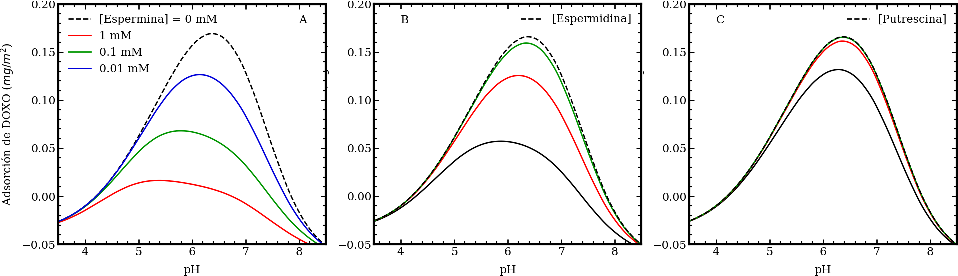
\includegraphics[width=0.9\textwidth]{Figures/graph-film/doxo_release-amines.pdf}
	\caption{Gr\'afico de la absorci\'on de la doxorrubicina (ver ecuaci\'on \ref{eq:film:adsorption}) en funci\'on del pH para soluciones que contienen espermina (A), espermidina (B) y putrescina (C).
		En cada panel, las diversas curvas s\'olidas corresponden a soluciones con diferentes concentraciones de poliamina, mientras que la curva discontinua corresponde a una soluci\'on sin poliaminas. Todos los resultados corresponden a soluciones de $1  \, mM$ de Doxo y $100\, mM$ de $NaCl$.}
	\label{fig:film:doxo-release}
\end{figure}



\begin{figure}[!htb]
	\centering
	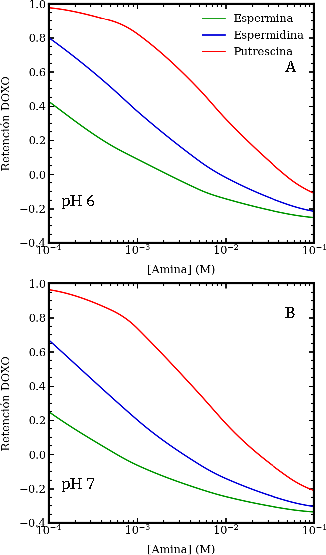
\includegraphics[width=0.45\textwidth]{Figures/graph-film/DG67.pdf}
	\caption{Gr\'afico que muestra la retenci\'on de Doxo, $\Gamma_{ret}$ (ver ecuaci\'on \ref{eq:film:doxo-DG}), en funci\'on de la concentraci\'on de aminas para soluciones con $100\, mM$ de $NaCl$ y un pH de 6 (panel superior) y pH de 7 (panel inferior). }
	\label{fig:film:doxo-DG}
\end{figure}

A continuaci\'on, evaluamos si la doxorrubicina puede liberarse del hidrogel cuando el material es\'a en contacto con soluciones de poliaminas. La figura \ref{fig:film:doxo-release} muestra la absorci\'on de Doxo en el film a partir de soluciones que contienen diferentes concentraciones de poliaminas. Como referencia, los gr\'aficos tambi\'en incluyen la absorci\'on de doxorrubicina a partir de soluciones que no contienen poliaminas. Nuevamente, consideramos una $[NaCl]$ fisiol\'ogica de $100\, mM$, pero ampliamos el rango de valores de pH para describir las condiciones que podr\'ian ocurrir alrededor de tejidos enfermos \'acidos. La absorci\'on de doxorrubicina es una funci\'on no monot\'onica del pH de la soluci\'on, con un m\'aximo entre $6$ y $7$. Este comportamiento no monot\'onico  era de esperar, ya que la carga neta negativa del pol\'imero es una funci\'on creciente del pH de la soluci\'on (ver figura \ref{fig:film:model}), mientras que la carga positiva promedio de la Doxo disminuye hasta volverse negativa eventualmente a valores de pH lo suficientemente altos (ver figura  \ref{fig:film:doxo-charge}).



\begin{figure}[!htb]
	\centering
	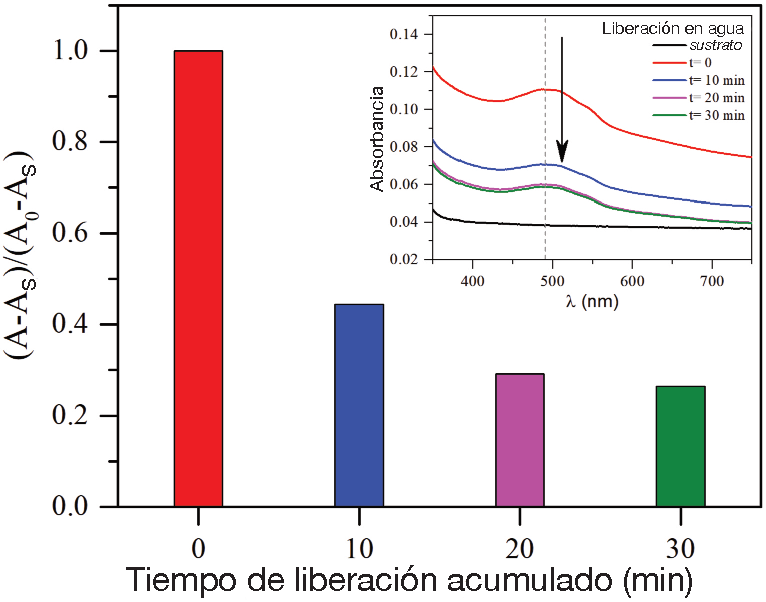
\includegraphics[width=0.45\textwidth]{Figures/graph-film/Release_water_2.pdf}
	\caption{Carga de doxorrubicina en films de PMAA y liberaci\'on de las mismas en agua, representada como el cambio en la absorbancia (a $\lambda=490 \,nm$) en relaci\'on con la carga inicial en diferentes tiempos de liberaci\'on.
		Inset: Gr\'afico de los espectros UV-Vis de los films despu\'es de 24 horas en contacto con Doxo (rojo; $t=0$).
		Las diversas curvas ilustran la liberaci\'on del f\'armaco despu\'es de diferentes tiempos de liberaci\'on en agua.
		La curva negra se incluye como referencia y corresponde a la se\~nal del soporte de vidrio desnudo. $A_s$: Absorbancia del sustrato de vidrio; $A_0$: Absorbancia del hidrogel completamente cargado. (Resultado experimental)}
	\label{fig:film:exp_doxo-water}
\end{figure}




La cantidad  de doxorrubicina en el film disminuye cuando las poliaminas est\'an presentes en la soluci\'on (compare las diferentes curvas de l\'inea s\'olida en la figura \ref{fig:film:doxo-release} con la curva de l\'inea discontinua en cada panel), lo cual se debe a la captura de poliaminas como se describe en la figura \ref{fig:film:amines-ads}. Esta disminuci\'on en la absorci\'on de Doxo en comparaci\'on con las soluciones sin el f\'armaco se puede interpretar como una liberaci\'on del material. Dado que la espermina es la el\'ectricamente  m\'as cargada, es la m\'as eficiente enfomentar  la desorci\'on de Doxo (ver panel A de la figura \ref{fig:film:doxo-release}).



\begin{figure*}[!ht]
	\centering
	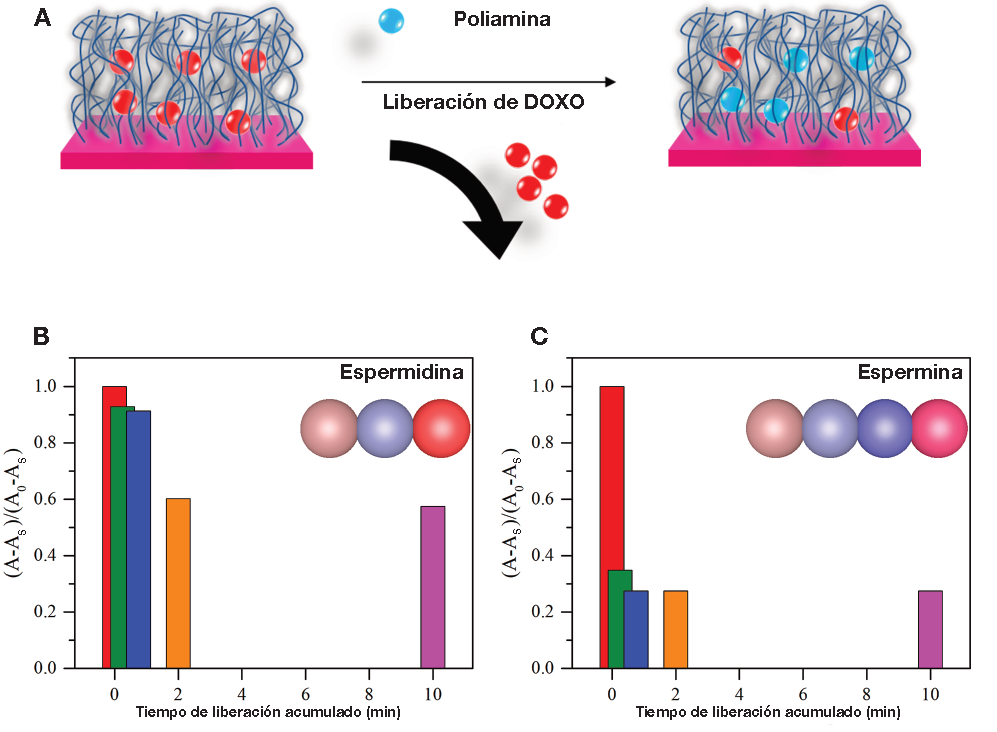
\includegraphics[width=0.7\textwidth]{Figures/graph-film/fig11.pdf}
	\caption{(A) Representaci\'on esquem\'atica de la liberaci\'on de Doxo mediante la absorci\'on de poliaminas. Carga y liberaci\'on de doxorrubicina en los films de PMAA en soluciones de espermina (B) y espermidina (C), representadas como el cambio en la absorbancia (a $\lambda=490 \, nm$) en relaci\'on con la carga inicial en diferentes momentos de liberaci\'on. $A_s$: Absorbancia del sustrato de vidrio; $A_0$: Absorbancia del hidrogel completamente cargado. (Resultados experimentales)}
	\label{fig:film:exp_doxo-amines}
\end{figure*}

Para cuantificar a\'un m\'as c\'omo el f\'armaco se desorbe de la pel\'icula de hidrogel cuando se incorporan aminas en la soluci\'on, definimos la reducci\'on relativa en la absorci\'on de doxorrubicina:


\begin{align}
	\begin{aligned}
		\Gamma_{ret}= \dfrac{\Gamma_\text{Doxo}([Amina])}{\Gamma_\text{Doxo}^0}
	\end{aligned}
	\label{eq:film:doxo-DG}
\end{align}


\noindent donde $\Gamma_{ret}$ es la retenci\'on de Doxo, $\Gamma_\text{Doxo}([Amina])$ es la absorci\'on de doxorrubicina para soluciones de amina (ver curvas de l\'inea s\'olida en la figura \ref{fig:film:doxo-release}), y $\Gamma_\text{Doxo}^0=\Gamma_\text{Doxo}([Amina]=0)$ es la absorci\'on en soluciones sin poliaminas (ver la figura \ref{fig:film:doxo-load} y las curvas de l\'inea discontinua en la figura \ref{fig:film:doxo-release}).

La figura \ref{fig:film:doxo-DG} muestra la retenci\'on de Doxo en presencia de cada una de las poliaminas en condiciones fisiol\'ogicas y a un pH de 6. Si todo el f\'armaco se mantiene dentro de la pel\'icula para una soluci\'on de poliamina, entonces $\Gamma_{ret}\approx 1$; mientras que $\Gamma_{ret}\approx 0$ indica que todo el f\'armaco ha sido liberado. Los valores negativos de $\Gamma_{ret}$ pueden ocurrir porque $\Gamma_\text{Doxo}([Amina])$, que es una cantidad en exceso en el bulk, puede tomar valores negativos, lo que indica que en esas condiciones las aminas evitan la absorci\'on de Doxo en la pel\'icula.

La retenci\'on de doxorrubicina en el hidrogel disminuye a medida que aumenta la concentraci\'on de poliamina. Esto es cierto para todas las aminas y para pH 7 y 6 (ver figura \ref{fig:film:doxo-DG}). Como se mencion\'o anteriormente, la espermina es la m\'as eficiente en promover la liberaci\'on de Doxo del hidrogel. Sin embargo, a altas concentraciones de amina, todas las poliaminas pueden impulsar la liberaci\'on de cantidades significativas de doxorrubicina.


\subsection{Espectro UV-Visible}

La carga de doxorrubicina en el hidrogel se caracteriz\'o mediante experimentos de UV-Vis, analizando la absorbancia a $\lambda=490\:$nm. Para abordar la liberaci\'on de Doxo despu\'es de la exposici\'on al agua, los datos de absorbancia se normalizaron en consecuencia, restando la absorbancia del sustrato de vidrio ($A_s$) y luego dividiendo por la absorbancia del hidrogel completamente cargado ($A_0$), tambi\'en con la resta de $A_s$. La figura \ref{fig:film:exp_doxo-water} muestra el cambio relativo en la absorbancia despu\'es de un tiempo de liberaci\'on dado para un hidrogel previamente cargado durante 24 h. El inset muestra los espectros UV-Vis despu\'es de diferentes tiempos de liberaci\'on en agua. Los resultados experimentales en $t=0$ (los espectros rojos mostrados en el inset de la figura \ref{fig:film:exp_doxo-water}) evidencian que las pel\'iculas de PMAA incorporan doxorrubicina dentro de su red polim\'erica. La absorbancia a $\lambda=490\, nm$ para ese espectro corresponde a la barra roja en la figura principal. Despu\'es de un tiempo de exposici\'on al agua lo suficientemente largo, la liberaci\'on de las pel\'iculas es solo parcial, lo que demuestra la afinidad del f\'armaco por la pel\'icula. Sin embargo, existe una clara y significativa liberaci\'on inicial del f\'armaco en los primeros 10 minutos, un comportamiento que no se observa en las etapas posteriores de liberaci\'on, donde las medidas se reducen a los mismos espectros (ver el inset de la figura \ref{fig:film:exp_doxo-water}).


La liberaci\'on de Doxo puede ser desencadenada al exponer la pel\'icula de hidrogel a poliaminas, como se representa en la figura \ref{fig:film:exp_doxo-amines}A. Para evaluar este comportamiento, se realizaron experimentos de liberaci\'on utilizando espermidina y espermina como poliaminas modelo. La  figura \ref{fig:film:exp_doxo-amines} muestra los cambios en la absorbancia relativa para las pel\'iculas de PMAA cargadas con Doxo y su liberaci\'on en contacto con soluciones de espermidina (panel B) y espermina (panel C) en diferentes tiempos de exposici\'on. La putrescina no se consider\'o en los experimentos debido a su baja absorci\'on en comparaci\'on con la espermina y la espermidina (ver figura \ref{fig:film:amines-ads}). Los resultados muestran que la liberaci\'on del f\'armaco en presencia de estas poliaminas es m\'as r\'apida que en agua, lo que respalda las predicciones de nuestra teor\'ia y modelado molecular: los hidrogeles de PMAA act\'uan como plataformas de absorci\'on para las poliaminas, y tal incorporaci\'on puede desencadenar la liberaci\'on de un f\'armaco previamente cargado.




La figura \ref{fig:film:exp_doxo-amines}, paneles  B y C, muestran que la liberaci\'on en presencia de espermina es m\'as r\'apida que con la incorporaci\'on de espermidina: despu\'es de una exposici\'on de 15 segundos a la espermina, ya no hay se\~nal UV de Doxo, mientras que se requiere un contacto tres veces m\'as largo con espermidina para alcanzar la misma etapa de liberaci\'on. Adem\'as, la magnitud de la liberaci\'on de Doxo utilizando espermidina es menos significativa en comparaci\'on con la liberaci\'on casi completa inducida por la espermina. Estos resultados indican que el n\'umero de grupos amino determina su retenci\'on en la pel\'icula de hidrogel, lo que concuerda con las predicciones de nuestra teor\'ia molecular (ver figura \ref{fig:film:doxo-DG}) y el trabajo de \citet{Schimka2017}.


\begin{figure}[!htb]
	\centering
	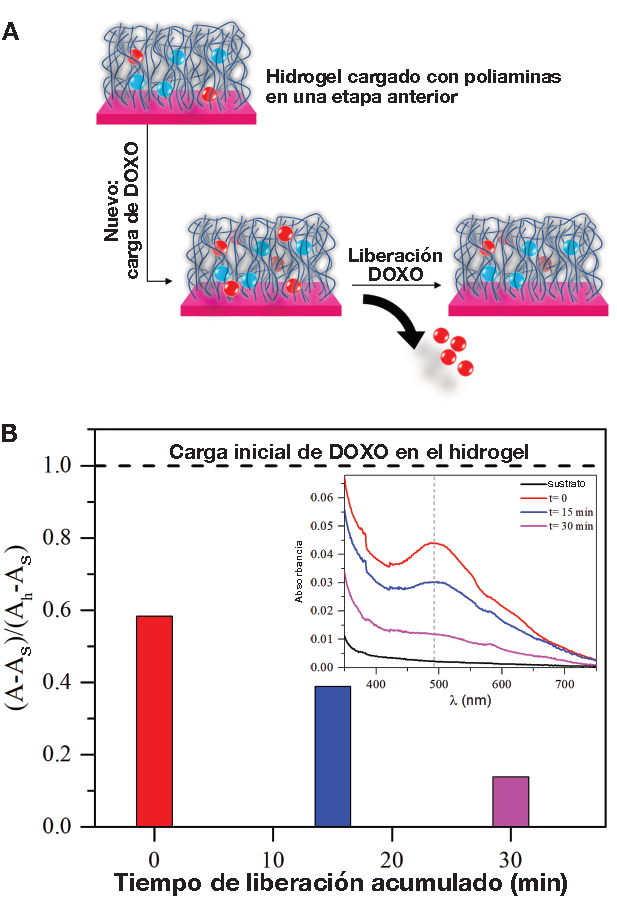
\includegraphics[width=0.45\textwidth]{Figures/graph-film/fig12.pdf}
	\caption{(A) Representaci\'on esquem\'atica de la recarga/liberaci\'on de Doxo despu\'es de la absorci\'on de poliaminas. (B) El cambio en la absorbancia (a $\lambda=490:$nm) en relaci\'on con la carga inicial de Doxo en el film de hidrogel (l\'inea discontinua). $A_s$: Absorbancia del sustrato de vidrio; $A_h$: Absorbancia de la carga inicial de Doxo en la pel\'icula de hidrogel (antes de la absorci\'on de poliaminas).}
	\label{fig:film:exp_doxo-reload}
\end{figure}


Despu\'es de la carga de poliaminas y la liberaci\'on concomitante de Doxo, las pel\'iculas de PMAA se expusieron a una nueva soluci\'on de Doxo para evaluar si la adsorci\'on de poliaminas impedir\'ia en la readsorci\'on de doxorrubicina, como se muestra en la figur \ref{fig:film:exp_doxo-reload}A. Estos experimentos tienen como objetivo responder si una vez liberada por la absorci\'on de poliaminas, la doxorrubicina se vuelve a adsorber en el hidrogel, disminuyendo su concentraci\'on en el medio. En l\'inea con el comportamiento esperado, la retenci\'on de espermina por la pel\'icula de hidrogel dificulta significativamente la reabsorci\'on de Doxo dentro de la red polim\'erica. Por otro lado, los films de hidrogel cargados con espermidina en contacto con Doxo muestran la posibilidad de recargar el f\'armaco, lo que sugiere una interacci\'on diferente, dependiendo de la poliamina. Como se muestra en el panel B de la figura \ref{fig:film:exp_doxo-reload}, la espermidina permite una recarga inicial de Doxo en el film, pero esta carga se libera f\'acilmente al medio, en comparaci\'on con los resultados de la figura \ref{fig:film:exp_doxo-water}, donde incluso despu\'es de 1 hora de exposici\'on al agua, el Doxo no se libera. Estos resultados tambi\'en resaltan la interacci\'on m\'as fuerte de la espermina (en comparaci\'on con la espermidina) con la red polim\'erica.

En resumen, nuestros resultados experimentales y te\'oricos muestran el potencial de los films de hidrogel basadas en PMAA para cargar f\'armacos terap\'euticos, que se explor\'o utilizando la Doxorrubicina como f\'armaco modelo. Si bien el hidrogel funciona como una plataforma de liberaci\'on controlada, la presencia de altas concentraciones de poliaminas en el medio circundante puede desencadenar la liberaci\'on del f\'armaco al interactuar con la red polim\'erica.



\section{Conclusiones}

Las poliaminas son esenciales para el metabolismo celular, ya que est\'an involucradas en diferentes procesos celulares y sirven como nutrientes para el crecimiento celular. En c\'elulas da\~nadas que muestran un crecimiento descontrolado, como los tumores, hay un aumento en la necesidad de nutrientes, lo que provoca un exceso medible en las concentraciones de poliaminas en los compartimentos extracelulares. Este aumento en la concentraci\'on de poliaminas juega un papel clave en la aceleraci\'on de la diseminaci\'on de tumores y puede servir como indicador de c\'elulas cancerosas. Concentraciones an\'omalas de poliaminas pueden ser la base para terapias que se centren en la eliminaci\'on de nutrientes y la prevenci\'on de met\'astasis, así\'i como para evaluar el avance de la quimioterapia.

En este contexto, nuestro objetivo en este trabajo fue demostrar el siguiente concepto: los hidrogeles basados en PMAA se pueden emplear para desarrollar biomateriales capaces de capturar poliaminas y liberar un f\'armaco terap\'eutico en respuesta. Hemos desarrollado un modelo molecular de grano grueso para describir la doxorrubicina, la putrescina, la espermidina y la espermina. Utilizando este modelo molecular y una teor\'ia termodin\'amica, nuestros resultados proporcionan informaci\'on sobre la adsorci\'on de poliaminas y doxorrubicina en pel\'iculas de hidrogel de PMAA.

Estos resultados predicen la capacidad de los hidrogeles de PMAA para capturar cantidades crecientes de poliaminas a medida que aumenta la concentraci\'on del medio en condiciones de sal fisiol\'ogicas. Esta absorci\'on aumenta con el n\'umero de grupos amino; la espermina muestra la preferencia m\'as fuerte por el hidrogel. Este comportamiento resulta de la interacci\'on entre la carga positiva de los grupos amino y los segmentos de MAA desprotonados (cargados negativamente).



Hemos considerado la carga de un f\'armaco contra el c\'ancer como la doxorrubicina en el hidrogel de PMAA. Las condiciones \'optimas de encapsulaci\'on en el laboratorio corresponden a una baja concentraci\'on de sal y un pH entre 6 y 7. Este resultado es contrario a la intuici\'on, ya que el punto isoelectroel\'ectrico de la doxorrubicina se encuentra alrededor de pH neutro. Este enfoque puede explicarse por la protonaci\'on del f\'armaco al adsorberse en el hidrogel en el medio de pH m\'as bajo.

Cuando tanto la doxorrubicina como una poliamina est\'an presentes en la soluci\'on en contacto con el hidrogel, las poliaminas dificultan significativamente la absorci\'on del f\'armaco (en comparaci\'on con las soluciones que contienen solo doxorrubicina). Este efecto se intensifica a medida que aumenta la concentraci\'on de poliaminas en la soluci\'on. La eficiencia para excluir el f\'armaco de la pel\'icula aumenta con la carga el\'ectrica  de la poliamina (es decir, el n\'umero de grupos amino); la espermina es la m\'as eficiente de las tres aminas consideradas para lograr esta respuesta. Como hemos demostrado, este comportamiento se puede interpretar como la liberaci\'on de doxorrubicina al capturar poliaminas.

Los films  de PMAA se sintetizaron mediante polimerizaci\'on radical de transferencia de \'atomos y se caracterizaron en condiciones espec\'ificas para respaldar nuestras predicciones te\'oricas. La absorci\'on y liberaci\'on de doxorrubicina en agua, soluciones de espermidina y espermina se estudiaron mediante espectroscopia UV-Vis. Estos resultados experimentales respaldan claramente el concepto propuesto de encapsulaci\'on de doxorrubicina dentro de estos films y la liberaci\'on de f\'armacos dependiente de poliaminas. % Utilizando las predicciones te\'oricas de este trabajo como gu\'ia, estamos trabajando actualmente en una caracterización sistemática del sistema experimental.

En resumen, nuestros estudios combinados te\'oricos y experimentales indican que los hidrogeles basados en \'acido polimetacr\'ilico tienen un gran potencial para servir como componente funcional en biomateriales que pueden capturar poliaminas y liberar un f\'armaco terap\'eutico en respuesta.